\section{Constraints on proton and nuclear structure}
\label{sec:protonPDFs}

By means of the strategy outlined in Sect.~\ref{sec:dis_pseudodata}, here
we quantify the impact on the proton PDFs
of differential  DIS
cross-section measurements exploiting the  LHC
neutrino beam. 
%
We assume an isoscalar free-nucleon target and neglect non-isoscalarity effects and nuclear modifications,
which are instead considered in Sect.~\ref{sec:nuclearPDFs}.
%
We present results first for the Hessian profiling of the PDF4LHC21,
and second for the Monte Carlo fit NNPDF4.0.
%
We study the stability of the results with respect to the inclusion of systematic uncertainties,
charm-tagged data, and lepton-charge separation.
%
We compare the impact of the different FPF experiments separately and also provide
results for their combination.

\subsection{Proton PDFs: impact on PDF4LHC21}
\label{sec:pdf4lhc21}

We begin by presenting results for the Hessian profiling of
the PDF4LHC21 NNLO set.
%
This proton PDF set is a Monte Carlo combination~\cite{Watt:2012tq,Carrazza:2015hva} of three global PDF sets, CT18~\cite{Hou:2019efy},
MSHT20~\cite{Bailey:2020ooq}, and NNPDF3.1~\cite{NNPDF:2017mvq}.
%
Its Hessian representations are obtained by means of the reduction methodologies developed in~\cite{Gao:2013bia,Carrazza:2015aoa}.
%
Being based on the combination of three modern global PDF fits, PDF4LHC21 provides a robust estimate
of  current uncertainties associated to our understanding of proton PDFs.
%
We profile PDF4LHC21 with pseudodata from various LHC neutrino experiments,
and study the stability of the results with respect to variations in the data
and methodology inputs.

%%%%%%%%%%%%%%%%%%%%%%%%%%%%%%%%%%%%%%%%%%%%%%%%%%%%%%%%%%%%%%%%%%%%%%%%
\begin{figure}[t]
\centering
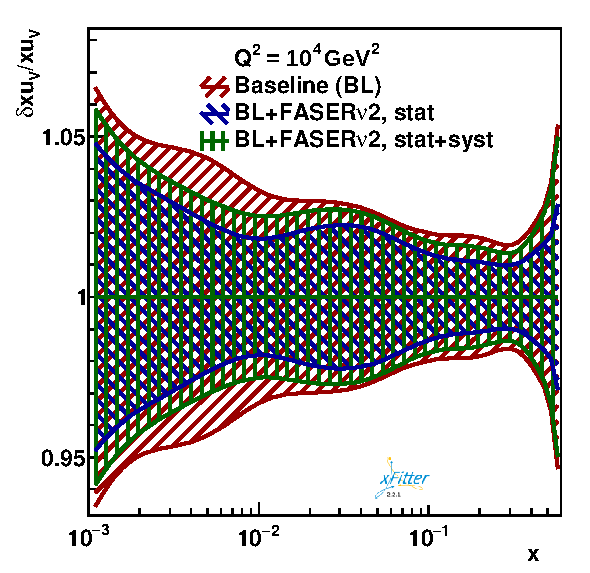
\includegraphics[width=0.32\textwidth]{plots/proton_fasernu2/inclusive+charm_chargediscrimination/fred05fcorr05_FASERv2_q2_10000_pdf_uv_ratio.pdf}
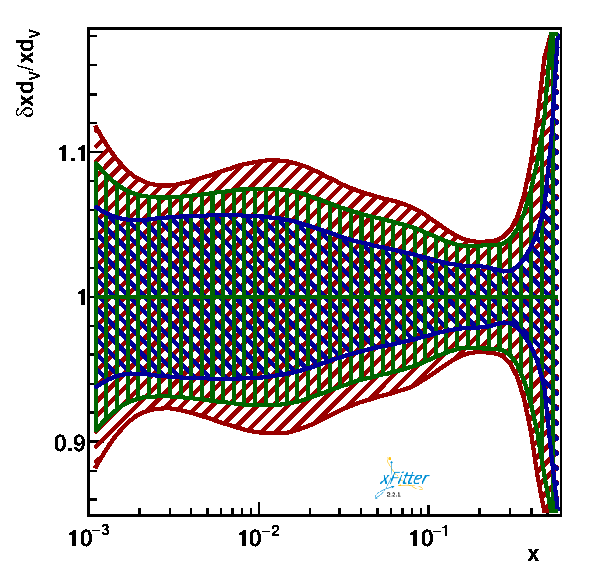
\includegraphics[width=0.32\textwidth]{plots/proton_fasernu2/inclusive+charm_chargediscrimination/fred05fcorr05_FASERv2_q2_10000_pdf_dv_ratio.pdf}
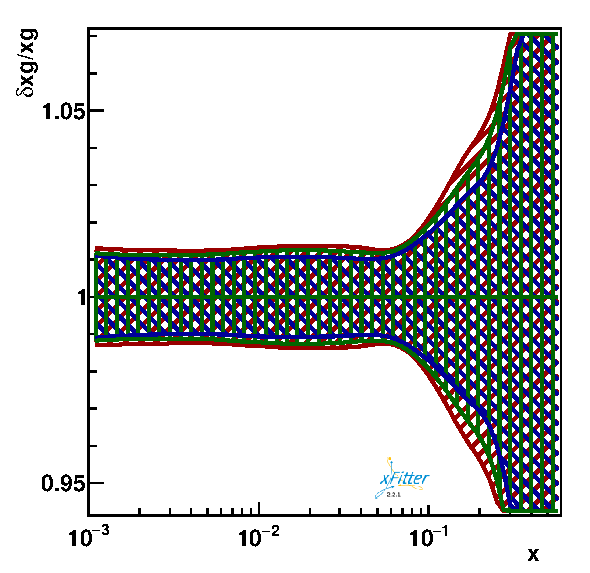
\includegraphics[width=0.32\textwidth]{plots/proton_fasernu2/inclusive+charm_chargediscrimination/fred05fcorr05_FASERv2_q2_10000_pdf_g_ratio.pdf}\\
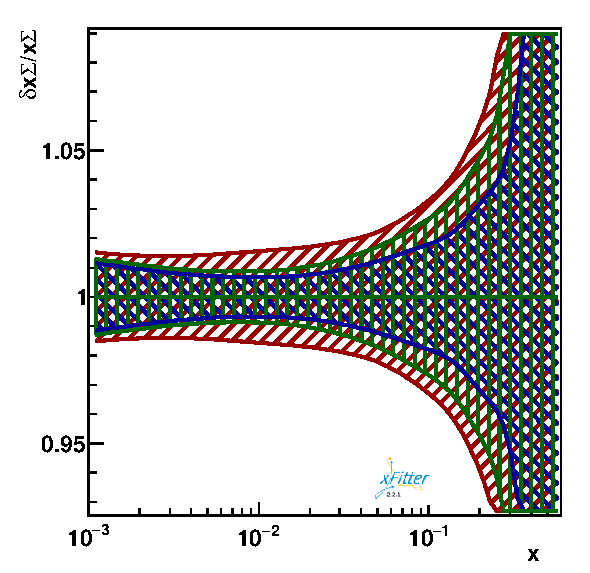
\includegraphics[width=0.32\textwidth]{plots/proton_fasernu2/inclusive+charm_chargediscrimination/fred05fcorr05_FASERv2_q2_10000_pdf_Sea_ratio.pdf}
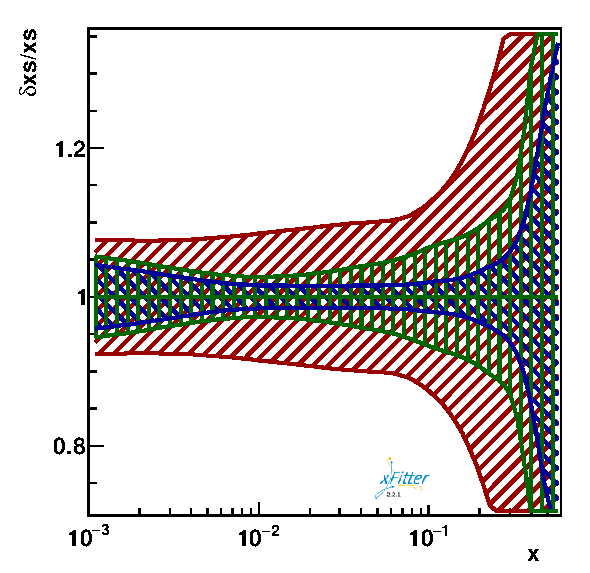
\includegraphics[width=0.32\textwidth]{plots/proton_fasernu2/inclusive+charm_chargediscrimination/fred05fcorr05_FASERv2_q2_10000_pdf_s_ratio.pdf}
\caption{
The fractional uncertainties (68\% confidence level) at $Q^2 = 10^4 \, \textrm{GeV}^2$ 
for the up and down valence quarks, gluon, total quark singlet, and total strangeness PDFs
in the PDF4LHC21 baseline, compared to the results obtained once the FASER$\nu$2 pseudo-data is included.
%
The FASER$\nu$2 impact projections are provided both without and with systematic
uncertainties accounted for.
%
We include  both  inclusive and charm-tagged structure functions
and assume outgoing lepton charge-separation.
%
}
\label{fig:FASERnu2_baseline}
\end{figure}
%%%%%%%%%%%%%%%%%%%%%%%%%%%%%%%%%%%%%%%%%%%%%%%%%%%%%%%%%%%%%%%%%%%%%%%%

\paragraph{Statistic versus systematic uncertainties.}
%
Fig.~\ref{fig:FASERnu2_baseline} shows the
fractional uncertainties (at the 68\% confidence level) at $Q^2 = 10^4 \, \textrm{GeV}^2$ 
for the up and down valence quarks, gluon, total quark singlet, and total strangeness PDFs
in the PDF4LHC21 baseline, compared to the results obtained once the FASER$\nu$2 pseudo-data is added
by means of Hessian profiling.
%
The FASER$\nu$2 pseudo-data accounts for  both  inclusive and charm-tagged structure functions
and assumes outgoing lepton- charge identification.
%
We display results for the profiling in which the experimental covariance matrix
considers only statistical uncertainties, as well as for the scenario where
statistical and systematic errors are added in quadrature following
the procedure spelled out in Sect.~\ref{subsec:uncertainties}.
%
We restrict the comparisons to the region $10^{-3}\lsim x \lsim 0.7$ covered
by the LHC neutrino experiments as shown in Fig.~\ref{fig:Kin_nNNPDF30_EIC_FPF}.
%
Note that in addition of a reduction of PDF uncertainties, the Hessian profiling
also results in general in a shift in the PDF central values.
%
This shift is however arbitrary since it 
depends on the fluctuations
entering the pseudo-data generation, and is hence ignored in the following.

Inspection of Fig.~\ref{fig:FASERnu2_baseline} reveals that measurements of DIS structure
functions at FASER$\nu$2 improve PDF uncertainties on the quark PDFs, while leaving
the gluon PDF essentially unaffected.
%
As expected for a neutrino scattering experiment, its impact is most marked for
those PDF combinations sensitive to quark flavour separation such as
the up and down valence PDF as well as the total strangeness.
%
Indeed, the reduction of PDF uncertainties is particularly significant for the latter,
a consequence of the inclusion of charm-tagged structure functions in the fit.
%
Given that all PDF determinations entering PDF4LHC21 already include existing neutrino
DIS measurements, the fact that FASER$\nu$2 pseudo-data still manages to reduce PDF
uncertainties highlights the new information provided by the LHC neutrino experiments.

By comparing the impact of the FASER$\nu$2 structure functions
in the case where only statistical errors are considered with that
where also systematic uncertainties are accounted for,
one finds that the latter eventually become a limiting factor,
but also that they not modify the qualitative findings of the statistics-only scenario.
%
Indeed, while systematic uncertainties somewhat degrade the PDF sensitivity,
they don't eliminate it for none of the quark PDFs.
%
Furthermore, in the projections presented in this work,
we assume the performance parameters of  Table~\ref{tab:FPF_experiments}, which
however could be very well enhanced in the actual realisation of the experiments,
using for instance detector improvements or different kinematic reconstruction techniques.
%
We also note that the availability of different experiments accessing the same neutrino
beam should allow their mutual cross-calibration, such that the combination of their
data brings in more information than just the trivial statistics scaling.

\paragraph{Importance of charm-tagged measurements.}
%
The analysis of Fig.~\ref{fig:FASERnu2_baseline} shows that LHC neutrino data is particularly
constraining for the poorly-known strange PDF, which is one of the quark flavour combinations
for which proton PDF fits differ the most~\cite{Faura:2020oom}.
%
To further investigate this point, Fig.~\ref{fig:FASERnu2_nocharm} compares the impact of the FASER$\nu$2 data shown in
Fig.~\ref{fig:FASERnu2_baseline}, for the case in which only statistical
uncertainties are considered, with the results of the same profiling once the charm-tagged
structure function data is excluded from the fit.
%
While differences are moderate for the up and down quark PDFs, the significant loss
of information resulting from this exclusion of charm-tagged data is clearly
visible for the strange PDF.
%
Specially in the region $x\gsim 0.01$, the constraints on strangeness shown in
Fig.~\ref{fig:FASERnu2_nocharm} are washed out in the absence of charm-tagged data.
%
We can hence establish that inclusive neutrino DIS measurements constrain mostly
the up and down quark and antiquark PDFs (and thus also the total quark singlet), while the charm-tagged
structure functions are responsible for most of the constraints provided on the total strangeness.
%
The PDF reach of the LHC neutrino experiments would thus be  markedly limited for experiments without
charm-identification capabilities.

%%%%%%%%%%%%%%%%%%%%%%%%%%%%%%%%%%%%%%%%%%%%%%%%%%%%%%%%%%%%%%%%%%%%%%%%
\begin{figure}[t]
\centering
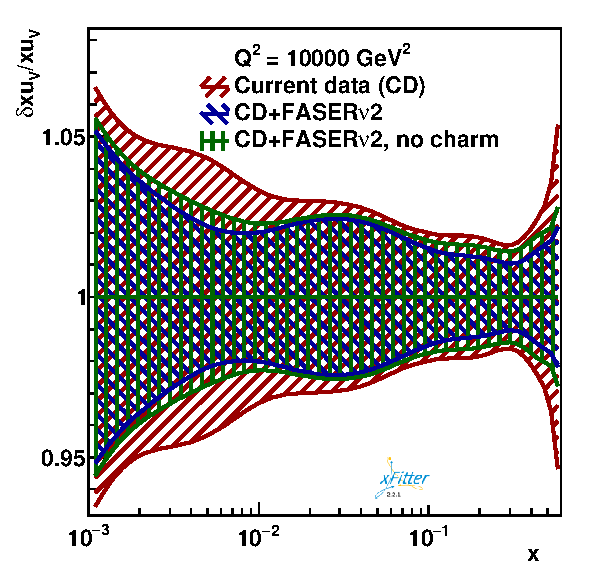
\includegraphics[width=0.32\textwidth]{plots/proton_fasernu2/inclusive-only_vs_inclusive+charm/statOnly_FASERv2_q2_10000_pdf_uv_ratio.pdf}
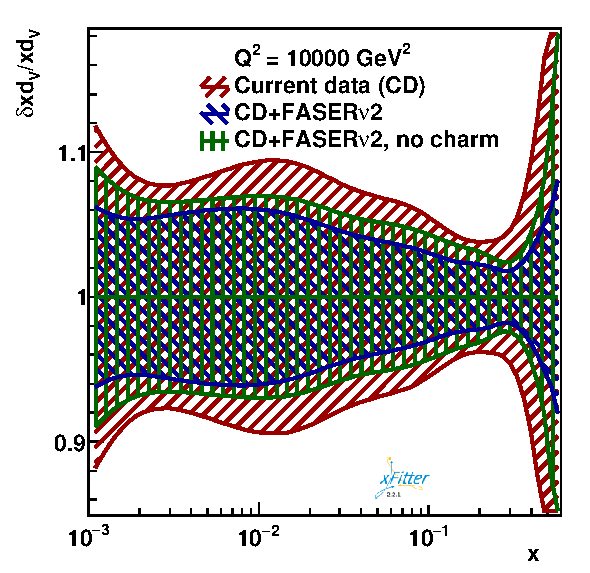
\includegraphics[width=0.32\textwidth]{plots/proton_fasernu2/inclusive-only_vs_inclusive+charm/statOnly_FASERv2_q2_10000_pdf_dv_ratio.pdf}
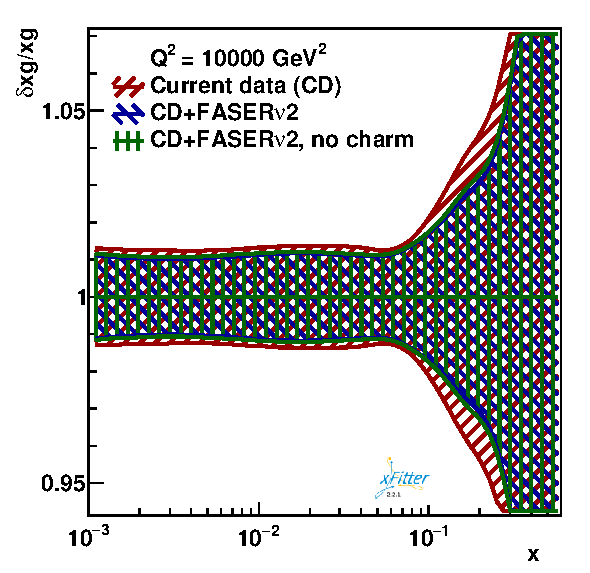
\includegraphics[width=0.32\textwidth]{plots/proton_fasernu2/inclusive-only_vs_inclusive+charm/statOnly_FASERv2_q2_10000_pdf_g_ratio.pdf}\\
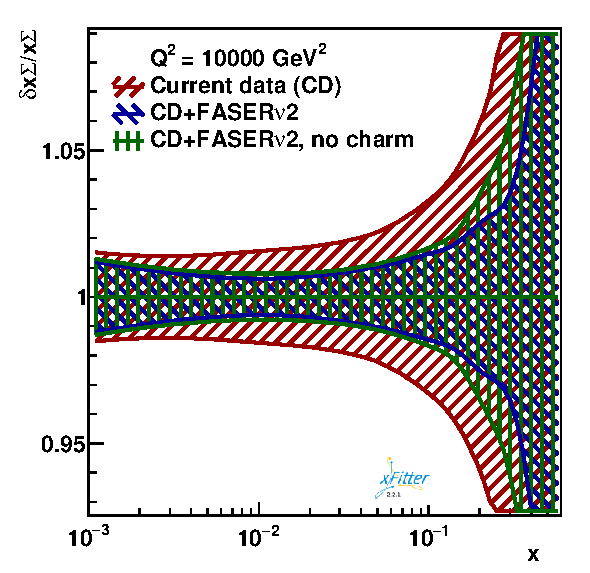
\includegraphics[width=0.32\textwidth]{plots/proton_fasernu2/inclusive-only_vs_inclusive+charm/statOnly_FASERv2_q2_10000_pdf_Sea_ratio.pdf}
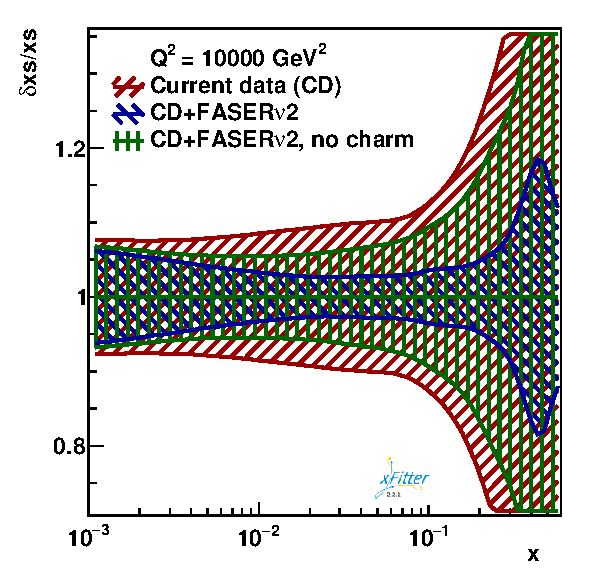
\includegraphics[width=0.32\textwidth]{plots/proton_fasernu2/inclusive-only_vs_inclusive+charm/statOnly_FASERv2_q2_10000_pdf_s_ratio.pdf}
\caption{Same as Fig.~\ref{fig:FASERnu2_baseline} (statistical uncertainties only),
  now showing results in the scenario where charm-tagged structure function measurements
  are excluded from the analysis.
}
\label{fig:FASERnu2_nocharm}
\end{figure}
%%%%%%%%%%%%%%%%%%%%%%%%%%%%%%%%%%%%%%%%%%%%%%%%%%%%%%%%%%%%%%%%%%%%%%%%

\paragraph{Lepton-charge identification.}
%
Being able to identify the charge of the produced final-state lepton in charged-current
neutrino scattering demands equipping an experiment with a powerful enough magnet suitable to
deflect this lepton within the detector fiducial volume.
%
Our baseline results for FASER$\nu$2 in Fig.~\ref{fig:FASERnu2_baseline} assume that this charge-identification
is possible, and therefore include separate structure function datasets for neutrino and anti-neutrino projectiles.
%
In order to ascertain to which extent the constraints provided by FASER$\nu$2 structure functions
depend on the availability of such a magnet,
Fig.~\ref{fig:FASERnu2_nochargeID} compares the reduction of the PDF uncertainties using
the FASER$\nu$2 data with and without charged-lepton identification capabilities.

%%%%%%%%%%%%%%%%%%%%%%%%%%%%%%%%%%%%%%%%%%%%%%%%%%%%%%%%%%%%%%%%%%%%%%%%
\begin{figure}[t]
\centering
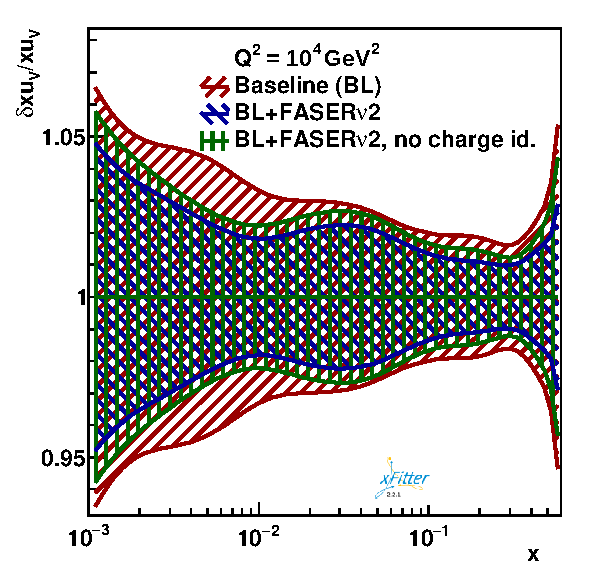
\includegraphics[width=0.32\textwidth]{plots/proton_fasernu2/nochargediscrimination/statOnly_FASERv2_q2_10000_pdf_uv_ratio.pdf}
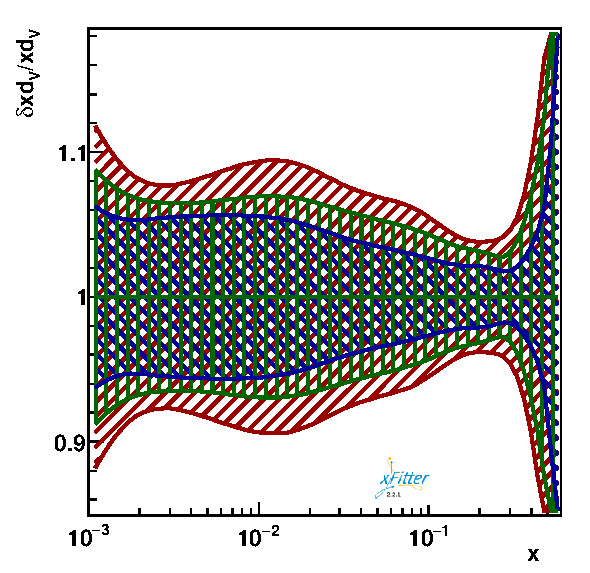
\includegraphics[width=0.32\textwidth]{plots/proton_fasernu2/nochargediscrimination/statOnly_FASERv2_q2_10000_pdf_dv_ratio.pdf}
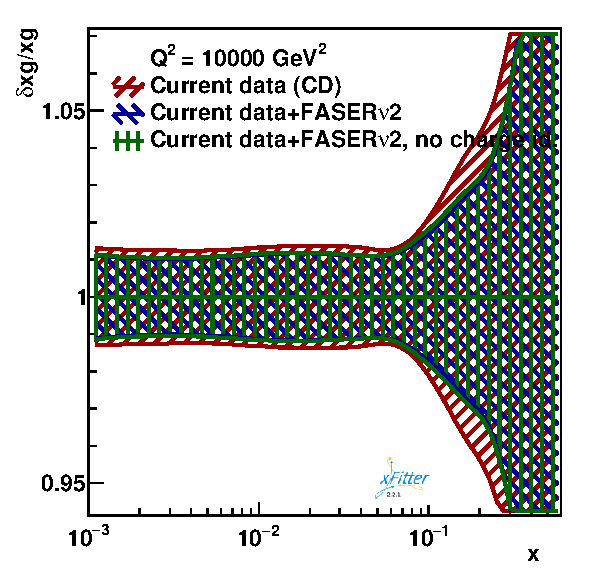
\includegraphics[width=0.32\textwidth]{plots/proton_fasernu2/nochargediscrimination/statOnly_FASERv2_q2_10000_pdf_g_ratio.pdf}\\
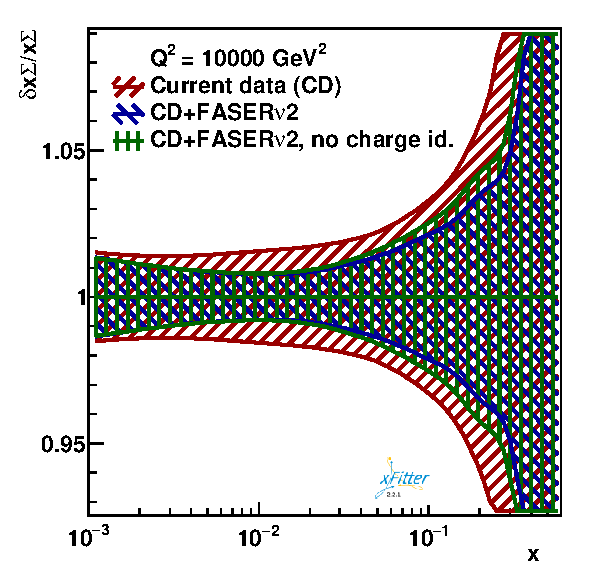
\includegraphics[width=0.32\textwidth]{plots/proton_fasernu2/nochargediscrimination/statOnly_FASERv2_q2_10000_pdf_Sea_ratio.pdf}
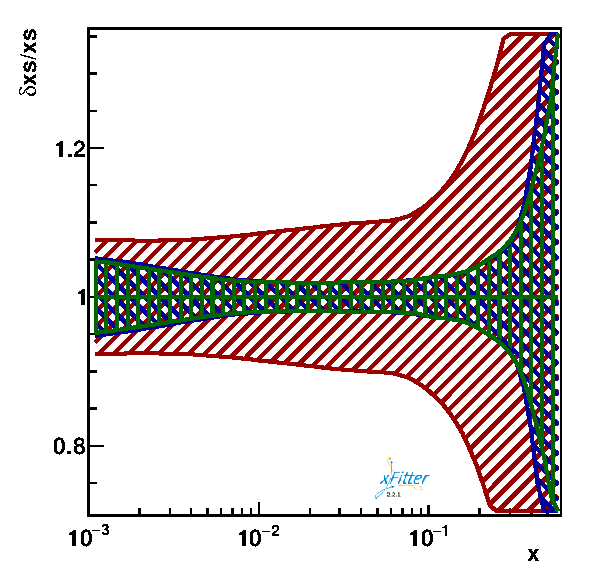
\includegraphics[width=0.32\textwidth]{plots/proton_fasernu2/nochargediscrimination/statOnly_FASERv2_q2_10000_pdf_s_ratio.pdf}
\caption{Same as Fig.~\ref{fig:FASERnu2_baseline} (statistical uncertainties only),
  now showing results in the scenario where the charge of the final-state charged lepton
  cannot be identified.
 }
\label{fig:FASERnu2_nochargeID}
\end{figure}
%%%%%%%%%%%%%%%%%%%%%%%%%%%%%%%%%%%%%%%%%%%%%%%%%%%%%%%%%%%%%%%%%%%%%%%%

One finds that the lack of charged-lepton identification actually does not degrade significantly the PDF
sensitivity of FASER$\nu$2.
%
Having access of the lepton charge information improves a bit the constraints for the down and (to a lesser
extent) the up valence quark PDFs,  while there are no differences for the total quark
singlet and for strangeness.
%
This behaviour can be understood by inspecting the leading-order decomposition of neutrino DIS
structure functions in terms of PDFs for different targets, Eqns.~(\ref{eq:neutrinoSFs_proton})--(\ref{eq:neutrinoSFs_isoscalar}).
%
For an isoscalar target, as assumed here, structure functions are very similar for neutrino
and anti-neutrino projectiles, with differences restricted to the strangeness asymmetry.
%
Given that this strangeness asymmetry is quite small, this also explains why the impact
on strangeness, which is driven by the charm-tagged data, is the same irrespective of whether one identifies
the outgoing lepton charge.
%
We conclude that LHC neutrino DIS data exhibits good PDF sensitivity even for an experiment which cannot tell
apart incoming neutrinos from antineutrinos.

\paragraph{FASER$\nu$2 compared to AdvSND and FLArE.}
%
In addition to FASER$\nu$2, we have also produced PDF impact projections for
other proposed FPF experiments, specifically for AdvSND and FLArE.
%
In the latter case, we consider both the 10 ton and 100 ton variants.
%
Figs.~\ref{fig:FASERnu2_advsnd} and~\ref{fig:FASERnu2_FLAre10} compare the PDF sensitivity
of FASER$\nu$2, in the scenario where systematic uncertainties are neglected, with the corresponding
results for AdvSND and FLArE100 respectively.
%
As summarised by Table~\ref{tab:integrated_rates}, each of these experiments
has associated different expected numbers of DIS events, namely 260k, 28k, and 57k (340K)
inclusive muon-neutrino events for FASER$\nu$2, AdvSND and FLArE10~(100) respectively,
with 39k, 3.5k, and 7.7k (45k) in the charm-tagged case.
%
In this comparison, one would expect that experiments with the largest event rates best PDF sensitivity.

%%%%%%%%%%%%%%%%%%%%%%%%%%%%%%%%%%%%%%%%%%%%%%%%%%%%%%%%%%%%%%%%%%%%%%%%
\begin{figure}[htbp]
\centering
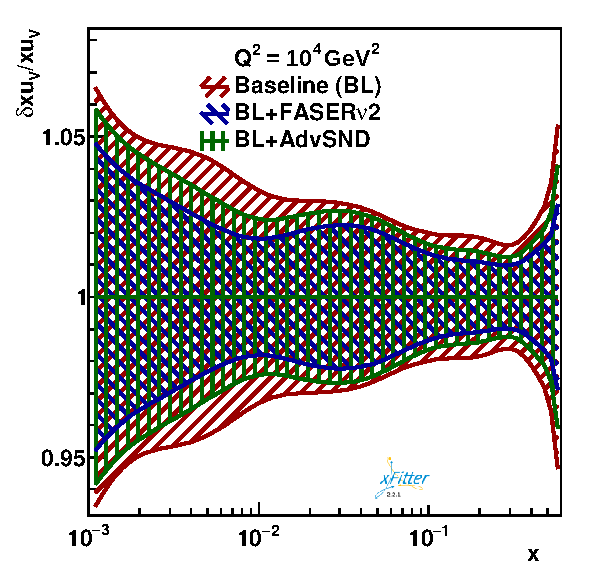
\includegraphics[width=0.32\textwidth]{plots/proton_fasernu2/FASERv2_vs_AdvSND/statOnly_AdvSND_q2_10000_pdf_uv_ratio.pdf}
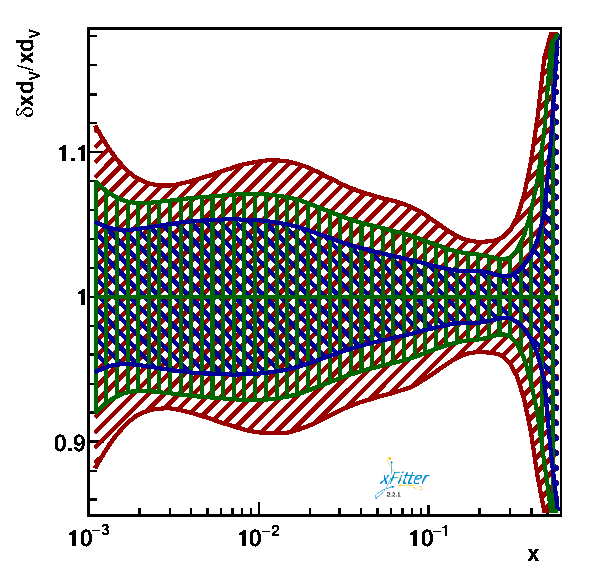
\includegraphics[width=0.32\textwidth]{plots/proton_fasernu2/FASERv2_vs_AdvSND/statOnly_AdvSND_q2_10000_pdf_dv_ratio.pdf}
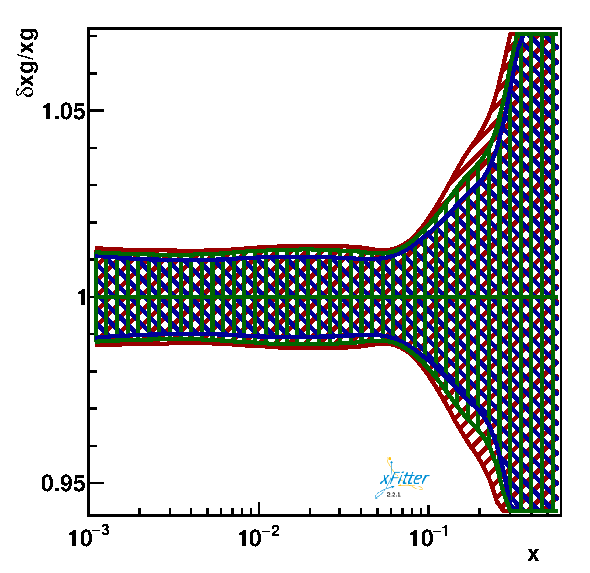
\includegraphics[width=0.32\textwidth]{plots/proton_fasernu2/FASERv2_vs_AdvSND/statOnly_AdvSND_q2_10000_pdf_g_ratio.pdf}\\
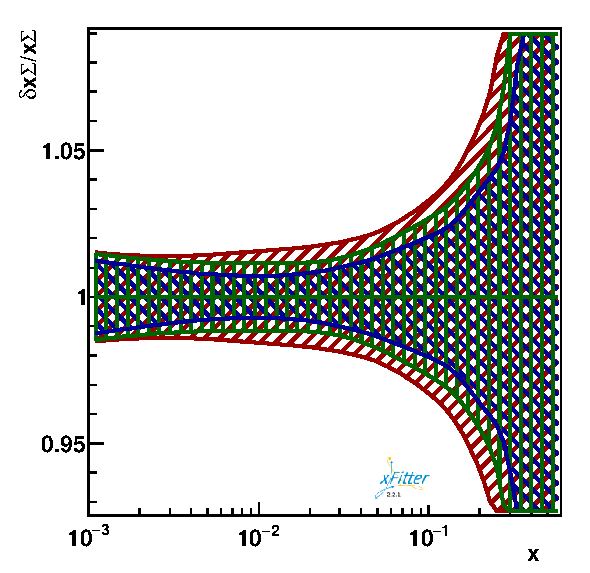
\includegraphics[width=0.32\textwidth]{plots/proton_fasernu2/FASERv2_vs_AdvSND/statOnly_AdvSND_q2_10000_pdf_Sea_ratio.pdf}
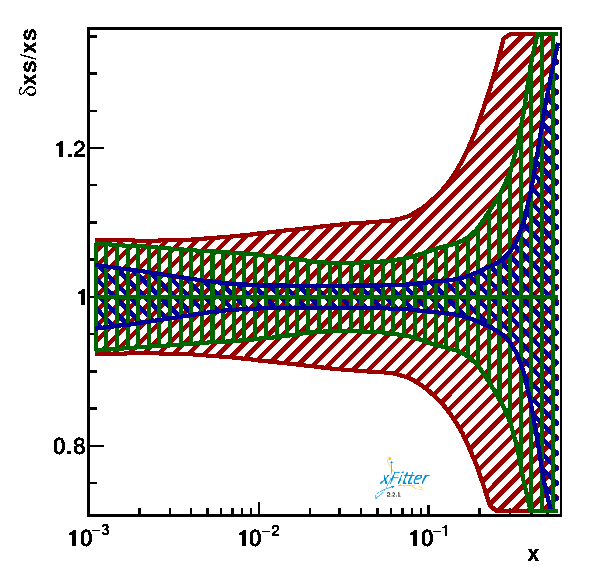
\includegraphics[width=0.32\textwidth]{plots/proton_fasernu2/FASERv2_vs_AdvSND/statOnly_AdvSND_q2_10000_pdf_s_ratio.pdf}\\
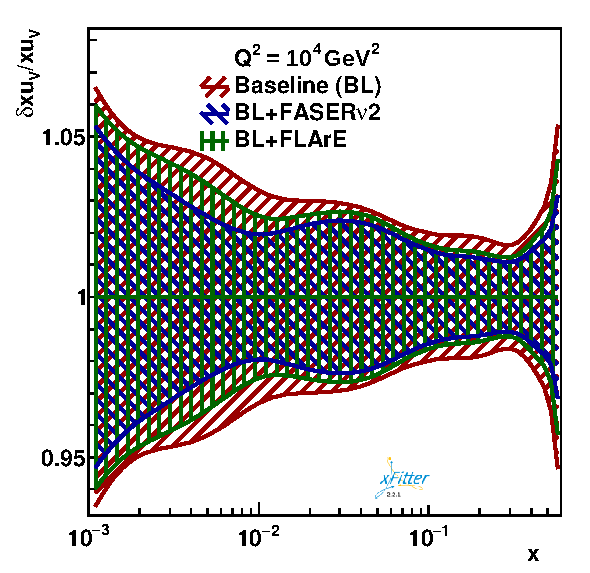
\includegraphics[width=0.32\textwidth]{plots/proton_fasernu2/FASERv2_vs_FLArE10/statOnly_FLArE10_q2_10000_pdf_uv_ratio.pdf}
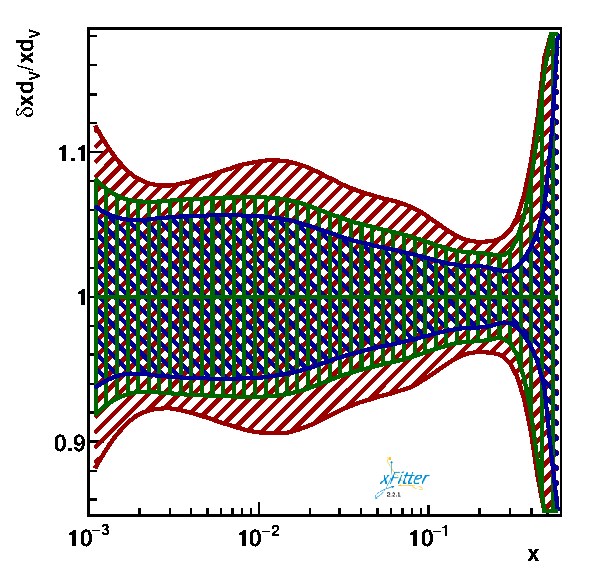
\includegraphics[width=0.32\textwidth]{plots/proton_fasernu2/FASERv2_vs_FLArE10/statOnly_FLArE10_q2_10000_pdf_dv_ratio.pdf}
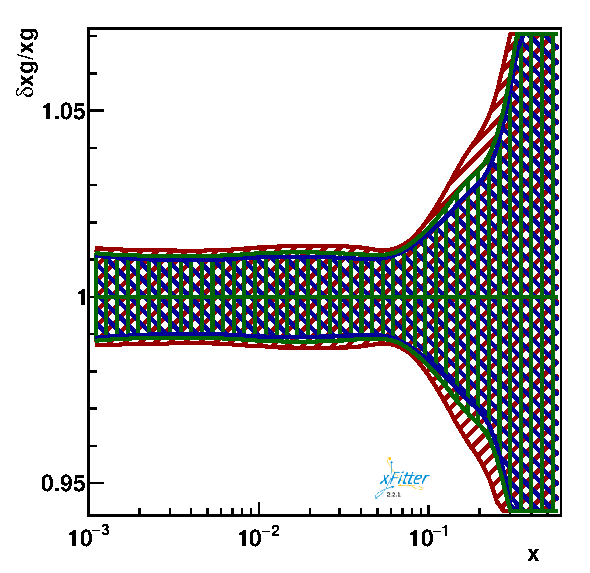
\includegraphics[width=0.32\textwidth]{plots/proton_fasernu2/FASERv2_vs_FLArE10/statOnly_FLArE10_q2_10000_pdf_g_ratio.pdf}\\
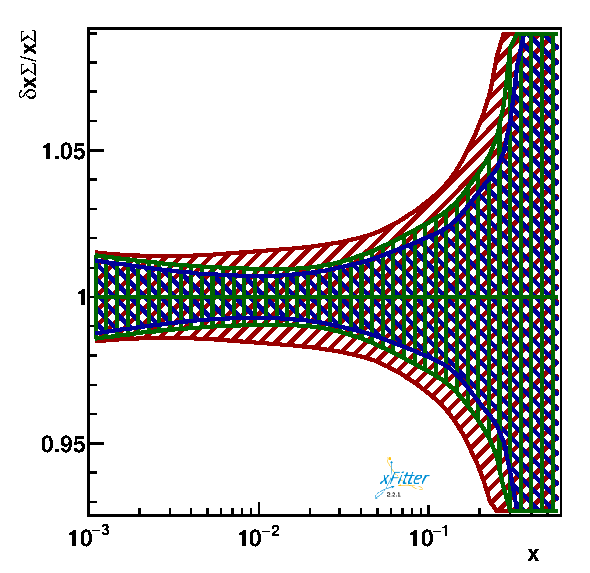
\includegraphics[width=0.32\textwidth]{plots/proton_fasernu2/FASERv2_vs_FLArE10/statOnly_FLArE10_q2_10000_pdf_Sea_ratio.pdf}
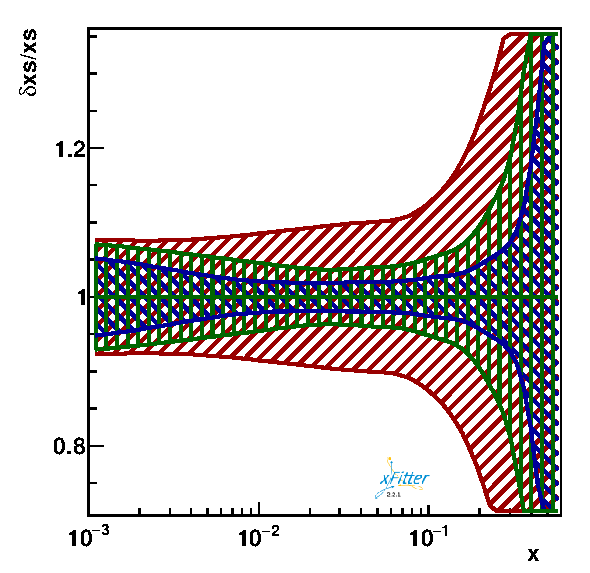
\includegraphics[width=0.32\textwidth]{plots/proton_fasernu2/FASERv2_vs_FLArE10/statOnly_FLArE10_q2_10000_pdf_s_ratio.pdf}
\caption{
  Same as Fig.~\ref{fig:FASERnu2_advsnd},
  comparing
  the projected PDF impact of FASER$\nu$2 with that of  AdvSND (top) and FLArE10 (bottom). 
}
\label{fig:FASERnu2_FLAre10}
\end{figure}
%%%%%%%%%%%%%%%%%%%%%%%%%%%%%%%%%%%%%%%%%%%%%%%%%%%%%%%%%%%%%%%%%%%%%%

From Figs.~\ref{fig:FASERnu2_advsnd} and~\ref{fig:FASERnu2_FLAre10} one can see that the three
FPF experiments studied lead to a reduction of the  uncertainties in the quark PDFs.
%
By comparing their relative impact, we find that the constraints
achieved by FASER$\nu$2 are somewhat better than for the other two experiments,
as could have been expected by the larger event yields obtained in the former.
%
In the case of AdvSND, the  smaller sample of charm-tagged events lead to reduction
of the constraints on strangeness.
%
Another consequence of the smaller event rates in AdvSND and FLArE10 as compared
to FASER$\nu$2 is the milder impact for the $x\lsim 10^{-2}$ region,
which can only be properly covered once the integrated statistics become large
enough,  as indicated by the differential bin-by-bin yields displayed in Fig.~\ref{fig:fasernu2_muon}.


We note that a proper comparison between the PDF reach of
the various FPF experiments requires accounting for the systematic uncertainties
associated to their kinematic reconstruction performance, which ultimately becomes
one of the limiting factors.
%
Also, as mentioned above, cross-calibration between experiments should provide
valuable input to enhance the PDF sensitivity.

\paragraph{Combined impact of the FPF experiments.}
%
Finally, we have carried out a further PDF analysis including simultaneously the three FPF experiments
considered so far: FASER$\nu$2, AdvSND, and FLArE100.
%
Fig.~\ref{fig:FPF_combined} displays the combined impact of the FPF experiments when added
on top of the  PDF4LHC21 baseline by means of Hessian profiling, both in the statistics-only case and
when systematic and statistical uncertainties are added in quadrature.
%
Possible correlations between the individual experiments are neglected in this exercise, though they
will become important when interpreting the actual measurements.

%%%%%%%%%%%%%%%%%%%%%%%%%%%%%%%%%%%%%%%%%%%%%%%%%%%%%%%%%%%%%%%%%%%%%%%
\begin{figure}[t]
\centering
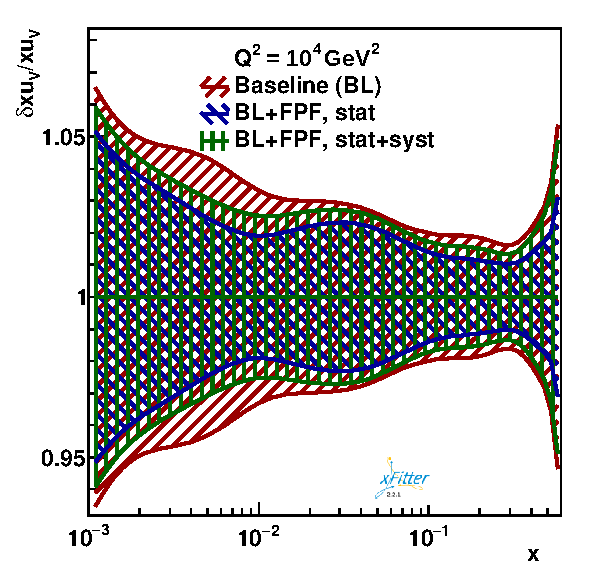
\includegraphics[width=0.32\textwidth]{plots/proton_fasernu2/FPF/fred05fcorr05_FPF_q2_10000_pdf_uv_ratio.pdf}
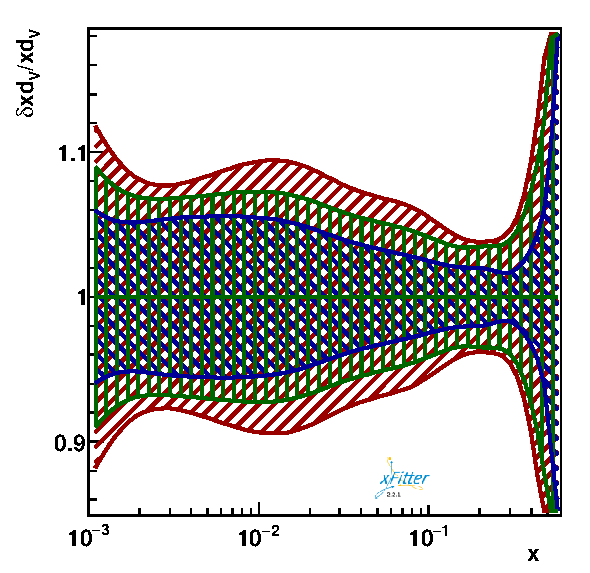
\includegraphics[width=0.32\textwidth]{plots/proton_fasernu2/FPF/fred05fcorr05_FPF_q2_10000_pdf_dv_ratio.pdf}
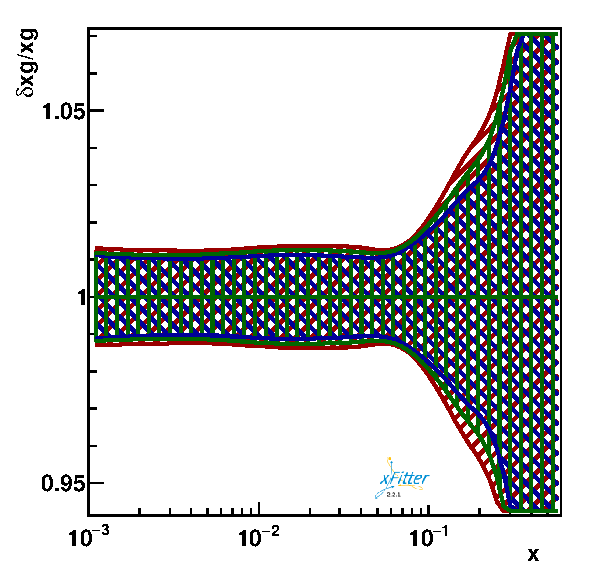
\includegraphics[width=0.32\textwidth]{plots/proton_fasernu2/FPF/fred05fcorr05_FPF_q2_10000_pdf_g_ratio.pdf}\\
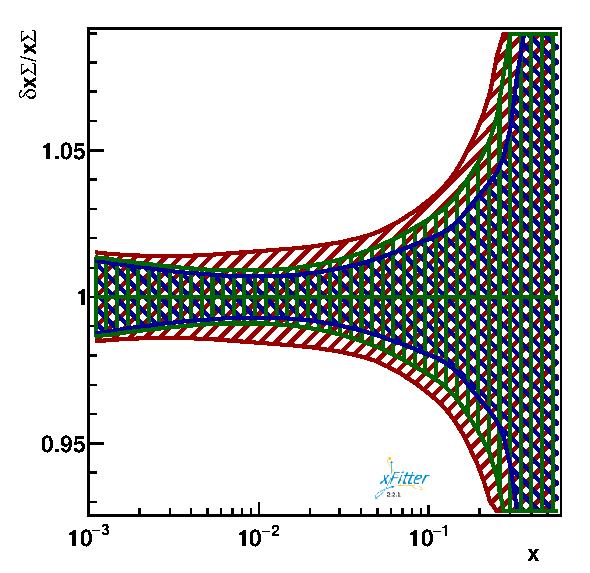
\includegraphics[width=0.32\textwidth]{plots/proton_fasernu2/FPF/fred05fcorr05_FPF_q2_10000_pdf_Sea_ratio.pdf}
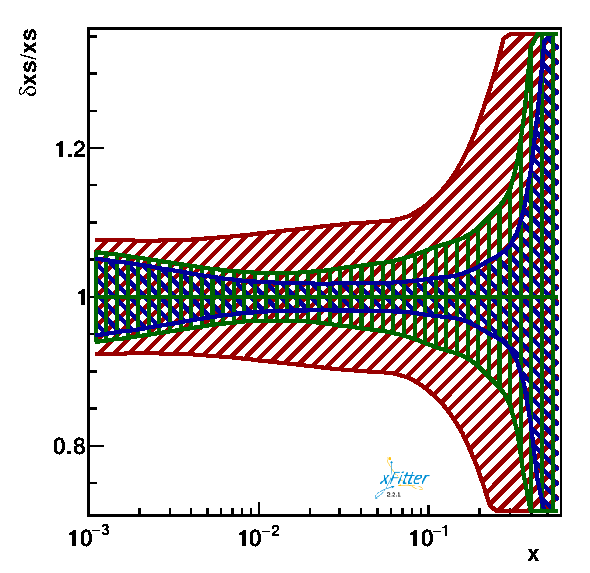
\includegraphics[width=0.32\textwidth]{plots/proton_fasernu2/FPF/fred05fcorr05_FPF_q2_10000_pdf_s_ratio.pdf}
\caption{
  Same as Fig.~\ref{fig:FASERnu2_baseline} now quantifying the
  projected PDF impact of the three FPF experiments added simultaneously to
  the analysis: FASER$\nu$2, AdvSND, and FLArE10. 
}
\label{fig:FPF_combined}
\end{figure}
%%%%%%%%%%%%%%%%%%%%%%%%%%%%%%%%%%%%%%%%%%%%%%%%%%%%%%%%%%%%%%%%%%%%%%%

The combined impact of the three FPF experiments on PDF4LHC21 shown in Fig.~\ref{fig:FPF_combined}
is only slightly improved as compared to the results of the FASER$\nu$2-only profiling
in Fig.~\ref{fig:FASERnu2_baseline}.
%
This shows that in this naive combination of experiments the one with the largest individual
sensitivity dominates, in this case FASER$\nu$2.
%
Again, this exercise is somewhat simplistic since within the real experiments the consistency (or lack thereof) between
individual measurements, which here is assumed by construction, provides useful information, and also
because the FPF experiments will cross-calibrate each other and cover somewhat different kinematic regions.

All in all, Fig.~\ref{fig:FPF_combined}, and in particular the statistics-only case, represents
a best-case scenario for the reduction of PDF uncertainties which can be expected from
the analysis of neutrino DIS structure function data at the FPF, in the assumption that PDF4LHC21 accurately represents
our current knowledge about the quark and gluon structure of the proton.

\subsection{Proton PDFs: impact on NNPDF4.0}
\label{sec:nnpdf40}

As discussed in Sect.~\ref{subsec:pdf_impact_assessment}, the PDF sensitivity
studies of the FPF neutrino data based on the {\sc\small xFitter} profiling
of PDF4LHC21 are complemented by those based on their direct inclusion
in the NNPDF4.0 global analysis.
%
Here we present results for the impact of the combined FPF neutrino
measurements on NNPDF4.0, namely the analogous study of that shown
in Fig.~\ref{fig:FPF_combined} in the case of PDF4LHC21.
%
We emphasize that we have produced results for the variations studied in
Sect.~\ref{sec:pdf4lhc21} also with the NNPDF fitting methodology.
%
Given that the qualitative obtained with the NNPDF fits
are compatible with those obtained with {\sc\small xFitter}, it is not necessary to duplicate them here,
and hence we only show results for the impact of the combined FPF pseudo-data.

Fig.~\ref{fig:NNPDF40_baseline} displays the
same results as Fig.~\ref{fig:FPF_combined} now in the case of the
fits obtained with the NNPDF4.0 fitting methodology.
%
The baseline NNPDF4.0 NNLO analysis is compared
with the results of the fits which include the combined FPF dataset,
in both the statistics-only scenario and for the case
where systematic uncertainties are also accounted for.
%
As in the PDF4LHC21 analysis, the bands indicate the one-sigma PDF uncertainties.
%
Note that we also show results for the charm PDF (bottom right panel), which
in the NNPDF4.0 fit is also determined directly from the data entering
the fit~\cite{Ball:2016neh}.
%
In this way, we can determine the possible constraints that neutrino
DIS measurements at the LHC may impose on the intrinsic charm
content of the proton~\cite{Ball:2022qks}.

 %%%%%%%%%%%%%%%%%%%%%%%%%%%%%%%%%%%%%%%%%%%%%%%%%%%%%%%%%%%%%%%%%%%%%%%%
\begin{figure}[t]
\centering
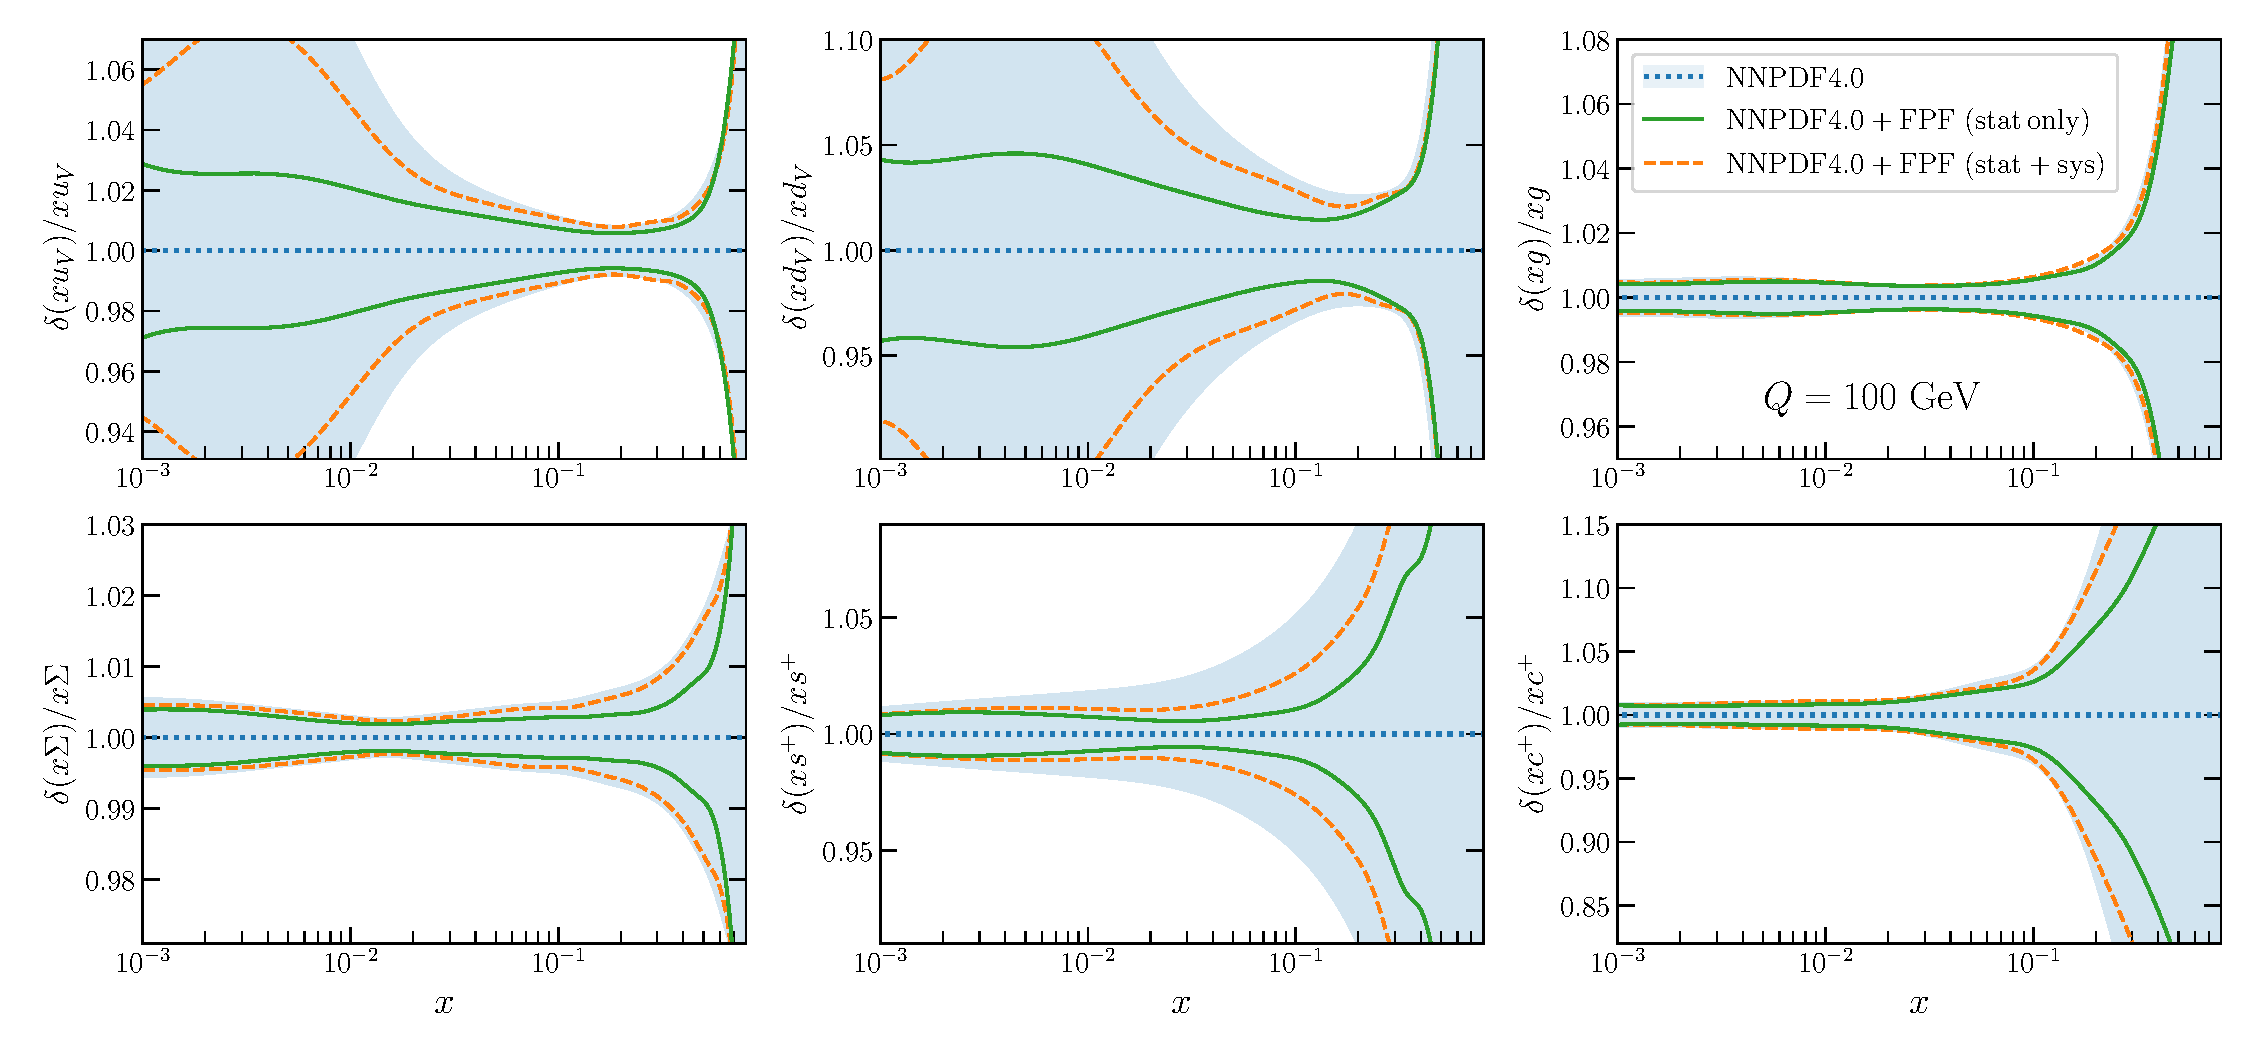
\includegraphics[width=0.99\textwidth]{plots/NNPDF40-FPFall-q100gev.pdf}
\caption{
  Same as Fig.~\ref{fig:FPF_combined} for the results obtained
  using the NNPDF4.0 fitting methodology.
  %
  The baseline NNPDF4.0 NNLO analysis is compared
  with the results of the fits which include the combined FPF dataset
  in both the statistics-only scenario and for the case
  where systematic uncertainties are also accounted for.
  %
  As in the PDF4LHC21 case, the bands indicate the one-sigma PDF uncertainties.
  %
  We now also show results for the charm PDF (bottom right panel), which
  in the NNPDF4.0 fit is also determined directly from the data entering the fit.
%
}
\label{fig:NNPDF40_baseline}
\end{figure}
%%%%%%%%%%%%%%%%%%%%%%%%%%%%%%%%%%%%%%%%%%%%%%%%%%%%%%%%%%%%%%%%%%%%%%%%

From  Fig.~\ref{fig:NNPDF40_baseline} one finds that
the impact on the PDFs found by direct inclusion of the FPF structure
functions on the NNPDF4.0 fit is qualitatively consistent with
that found in the the Hessian profiling of PDF4LHC21.
%
In particular, the constraints are more significant for the up and down
quark valence PDFs as well as for the total strangeness.
%
As was the case with the PDF4LHC21 baseline, the uncertainty reduction
for the strangeness PDF is particularly
striking.
%
Also consistently with the results of Sect.~\ref{sec:pdf4lhc21}, the gluon
PDF is unchanged, and the impact on the total quark PDF
is restricted to the large-$x$ region.
%
While one can also identify differences related to analysis choices
such as the PDF parametrisation and the method used to assess the PDF
error reduction (for example, concerning the small-$x$ behaviour of $xu_V$ and $xd_V$)
we conclude that by and large the projected impact of the FPF structure function
measurements is independent of the specific fitting methodology adopted.

 %%%%%%%%%%%%%%%%%%%%%%%%%%%%%%%%%%%%%%%%%%%%%%%%%%%%%%%%%%%%%%%%%%%%%%%%
\begin{figure}[t]
\centering
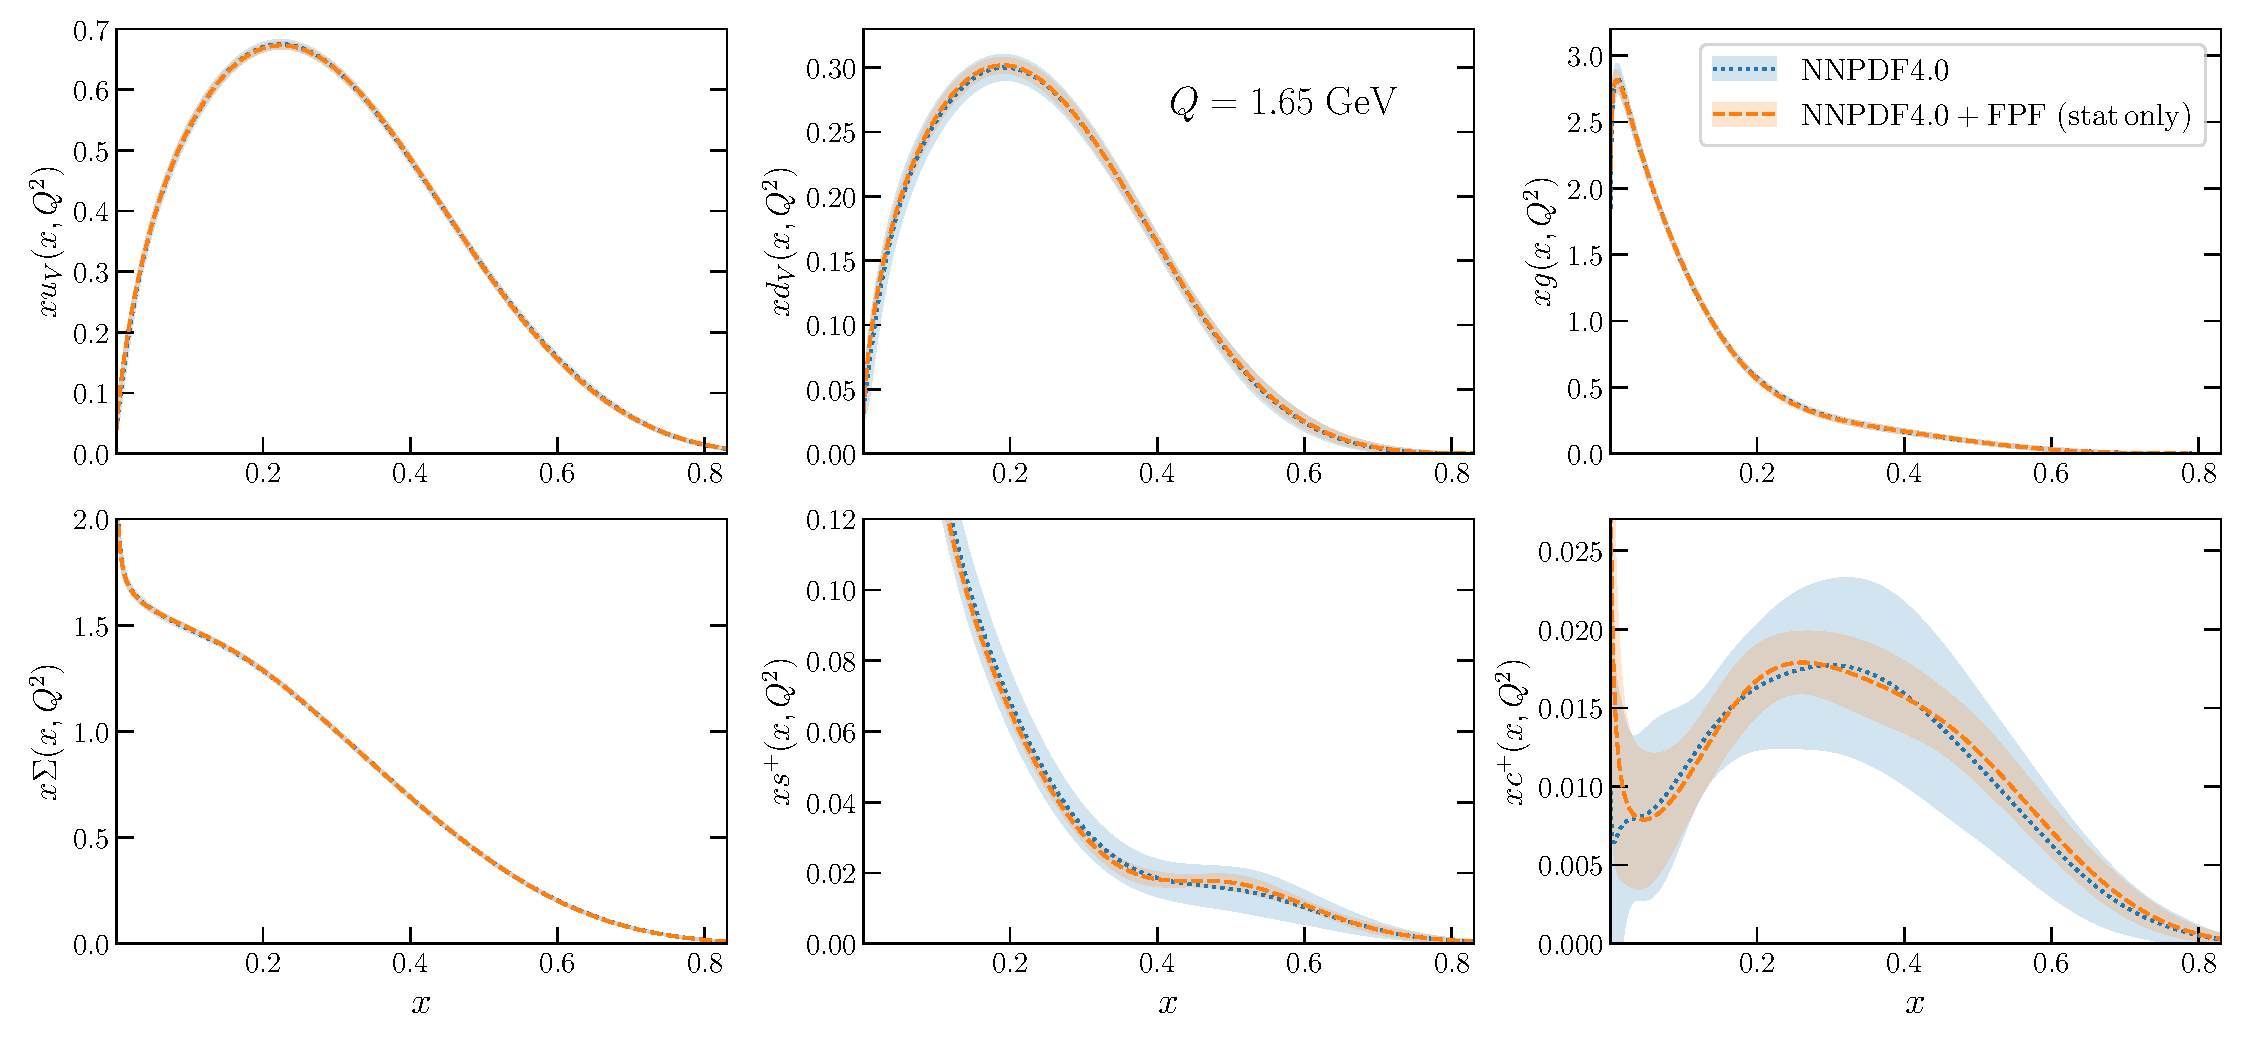
\includegraphics[width=0.99\textwidth]{plots/NNPDF40-FPFall-q1p65gev-abs.pdf}
\caption{
  Same as Fig.~\ref{fig:NNPDF40_baseline} now for the absolute PDFs
  at the initial parametrisation scale, $Q=1.65$ GeV, focusing
  on the large-$x$ region.
%
}
\label{fig:NNPDF40_lowQ_abs}
\end{figure}
%%%%%%%%%%%%%%%%%%%%%%%%%%%%%%%%%%%%%%%%%%%%%%%%%%%%%%%%%%%%%%%%%%%%%%%%

As indicated by Fig.~\ref{fig:NNPDF40_baseline}, the FPF data is also expected
to reduce the uncertainties associated to the fitted charm PDF in the region $x\simeq 0.2$
dominated by the non-perturbative component.
%
In order to highlight this impact on the large-$x$ region of the PDFs,
Fig.~\ref{fig:NNPDF40_lowQ_abs} presents the same comparison as
in  Fig.~\ref{fig:NNPDF40_baseline} now for the absolute PDFs
at the initial parametrisation scale, $Q=1.65$ GeV, using a linear scale, for the statistics-only
scenario.
%
One can observe the improved constraints on the charm PDF in the large-$x$ region,
further confirming previous studies~\cite{Anchordoqui:2021ghd,Feng:2022inv} that indicate the
sensitivity of the FPF to the intrinsic charm content of the proton.
%
This comparison also illustrates the excellent constraining power on the proton
strangeness enabled by the FPF charm-tagged structure function data.

%-----------------------------------------------------------------------
\begin{table}[!t]
  \centering
  \footnotesize
  \renewcommand{\arraystretch}{1.30}
  \begin{tabularx}{\textwidth}{X|l|c|c|c}
  \toprule
  & \multirow{3}{*}{Dataset}
  & \multicolumn{3}{c}{\bf NNPDF4.0 NNLO} \\
  &
  & \multirow{2}{*}{Baseline}
  & \multicolumn{2}{c}{with combined FPF data}  \\
  &
  &
  & Statistical-only  & Statistical + systematics  \\
  \midrule
  $\chi^2$ &  \multirow{4}{*}{Global}  & 1.170 &  1.161  & 1.145  \\
  $\la E_{\rm tr}\ra_{\rm rep}$
  &  &  2.256  &  2.242   & 2.215   \\
  $\la E_{\rm val}\ra_{\rm rep}$
  & & 2.360    &   2.332  & 2.311  \\
  $\la \chi^2\ra_{\rm rep}$
  & &   1.194   &    1.187    & 1.169  \\
  \midrule
  \multirow{8}{*}{$\chi^2$}
  & DIS neutral-current                     &  1.220    &  1.230    &   1.220   \\
  & DIS charged-current                     &   0.904  &   0.942    &  0.913    \\
  & Drell--Yan (inclusive and one-jet) &  1.76   &   1.830    &   1.830   \\
  & Top-quark pair production               &  1.230   &   1.220    &  1.250    \\
  & Single-top production                   &  0.362   &   0.364    &   0.361   \\
  & Inclusive jet production                &  0.957   &  0.963     &   0.942   \\
  & Dijet production                        &  2.030    &    2.010   &   2.010   \\
  & Direct photon production                 &  0.740  &   0.729    &    0.744  \\
  & FPF (total)                 &  -  &       &      \\
  \bottomrule
\end{tabularx}
\vspace{0.2cm}
\caption{\small Statistical estimators for the NNPDF4.0 NNLO
  baseline fit, compared to the variants including
  the combined FPF dataset shown in Figs.~\ref{fig:NNPDF40_baseline}
  and~\ref{fig:NNPDF40_lowQ_abs}.
  %
  From top to bottom: total $\chi^2$, average
  over replicas of the training and validation figures of merit
  $\la E_{\rm tr}\ra_{\rm rep}$ and $\la E_{\rm val}\ra_{\rm rep}$,
  average $\chi^2$ over replicas $\la \chi^2\ra_{\rm rep}$,
  $\chi^2$ for datasets grouped by process.
  %
  The last row displays the $\chi^2$ obtained for the combined FPF dataset.
  \label{tab:chi2_nnpdf40_baseline}
}
\end{table}
%--------------------------------------------------------------------------

The statistical estimators for the NNPDF4.0 NNLO
baseline fit, compared to the variants including
the combined FPF dataset shown in Figs.~\ref{fig:NNPDF40_baseline}
and~\ref{fig:NNPDF40_lowQ_abs}, are reported in Table~\ref{tab:chi2_nnpdf40_baseline}.
%
From top to bottom we indicate the total $\chi^2$, average
over replicas of the training and validation figures of merit
$\la E_{\rm tr}\ra_{\rm rep}$ and $\la E_{\rm val}\ra_{\rm rep}$,
average $\chi^2$ over replicas $\la \chi^2\ra_{\rm rep}$,
$\chi^2$ for datasets grouped by process.
%
Note that the last row displays the $\chi^2$ obtained for the combined FPF dataset.
%
For the latter, one finds that as expected $\chi^2 \sim 1$, given that the FPF pseudo-data
is produced by construction to be fully compatible with the NNPDF4.0 baseline.
%
For the same reason, the description of all other experiments entering
the NNPDF4.0 global fit is not distorted by the inclusion of the FPF data.
%
In particular, the $\chi^2$ of the available (non-FPF) DIS neutral-current and charged-current
datasets changes from 1.220 and 0.904 in NNPDF4.0 to 1.220 and 0.913 in the fit
with FPF pseudo-data.
%
A moderate increase is found to the $\chi^2$ of Drell-Yan processes, from 1.76 to 1.83, possibly
because of the enhanced weight that DIS data carries in this fit variant.

Fig.~\ref{fig:nnpdf40_fpf_lumis} displays a comparison of the PDF luminosities at $\sqrt{s}=14$ TeV
as a function of the final-state invariant mass $m_X$ between
the baseline NNPDF4.0 NNLO determination and its variant which includes
the combined FPF pseudo-data from the FASER$\nu$2, FLArE100, and AdvSND experiments,
see Figs.~\ref{fig:NNPDF40_baseline} or the corresponding PDF comparison.
%
%
  Results are shown normalised to the central value of the NNPDF4.0 baseline.
  %
  Specifically, we show the gluon-gluon, quark-antiquark, and
  quark-quark luminosities.
  %
These luminosities are useful to interpret the phenomenological studies with the FPF-improved
PDFs for the HL-LHC that will be presented in Sect.~\ref{sec:pheno}.

%%%%%%%%%%%%%%%%%%%%%%%%%%%%%%%%%%%%%%%%%%%%%%%%%%%%%%%%%%%%%%%%%%%%%%%%
\begin{figure}[t]
\centering
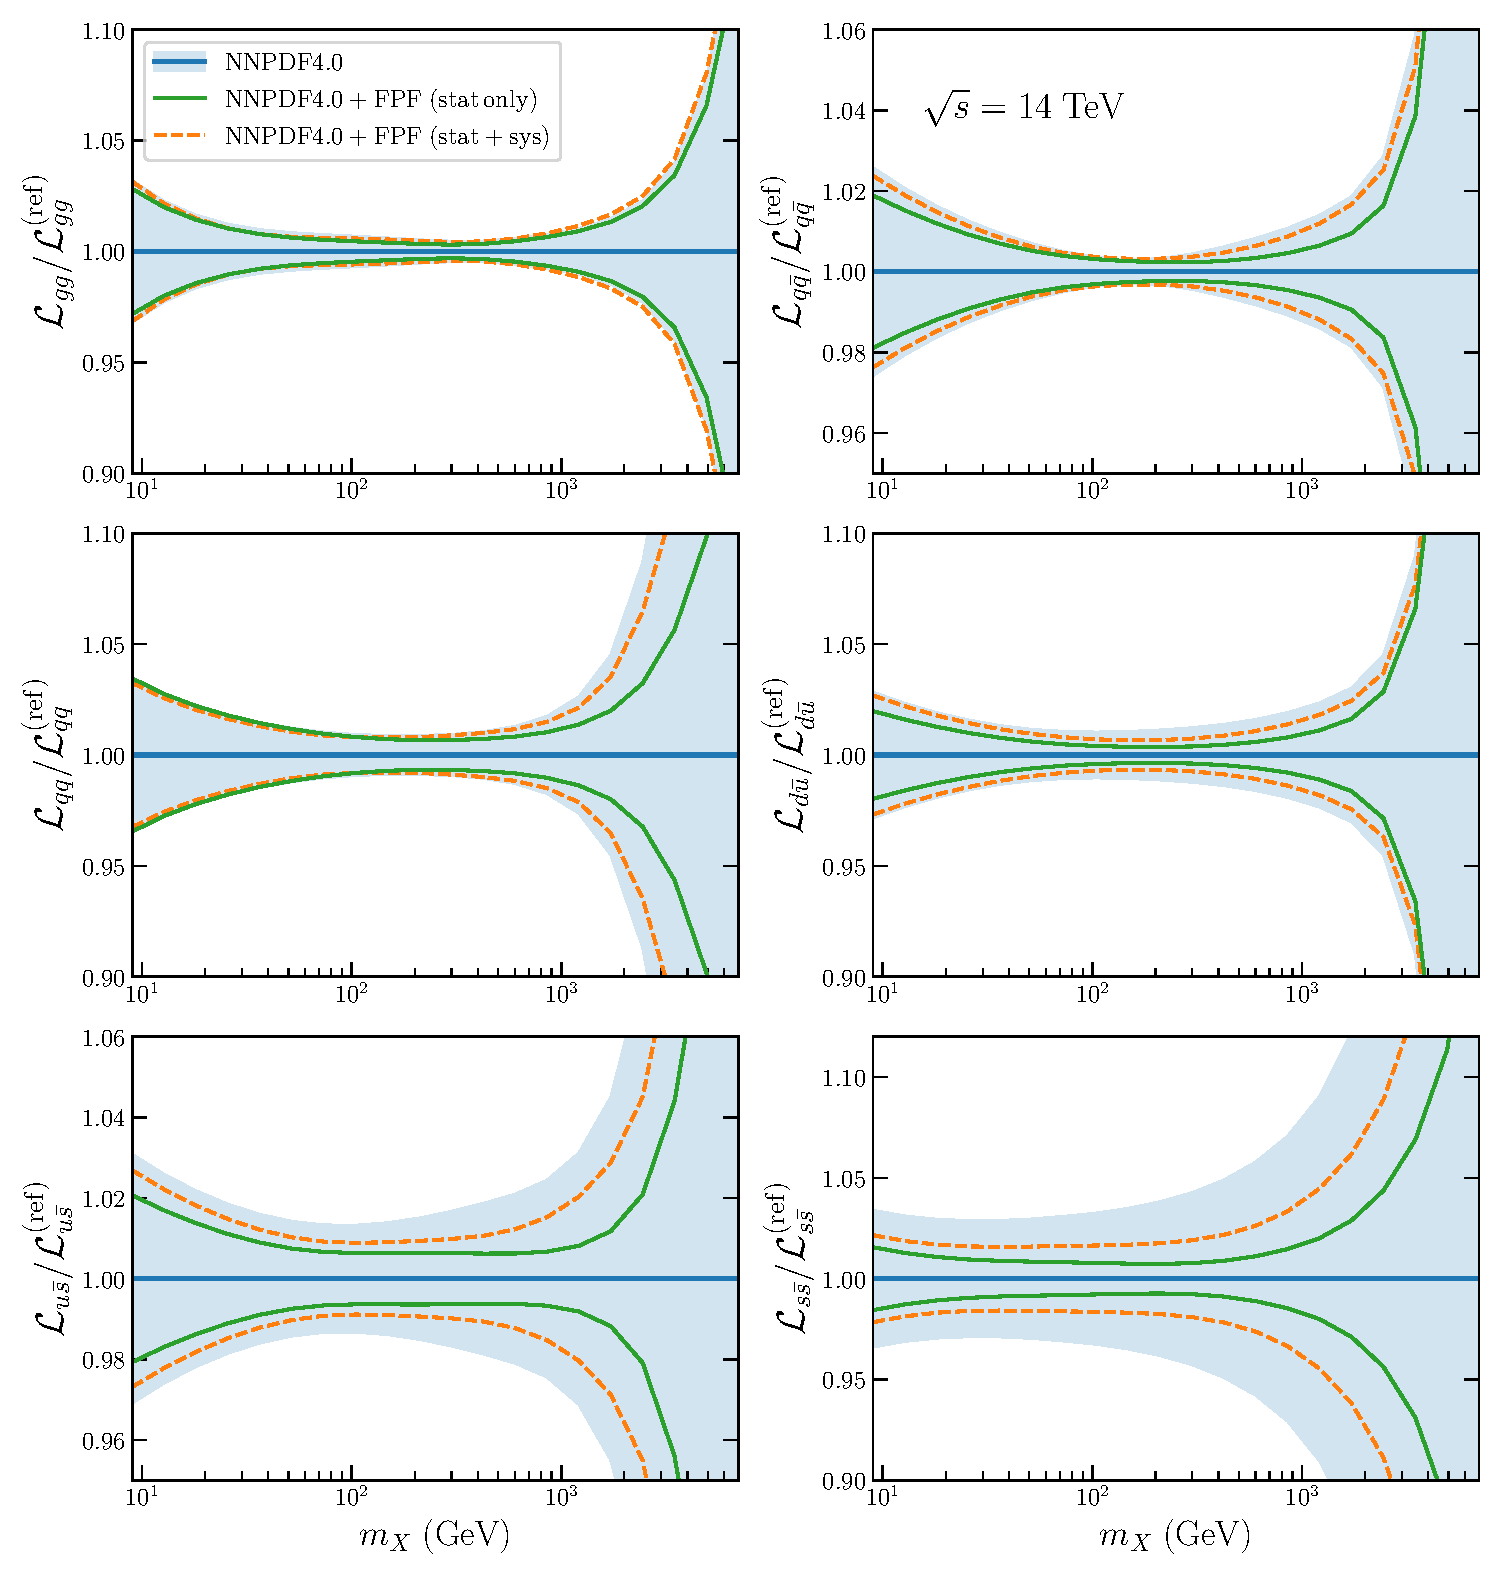
\includegraphics[width=0.99\textwidth]{plots/lumi-FPFall.pdf}
\caption{Comparison of the PDF luminosities at $\sqrt{s}=14$ TeV
  as a function of the final-state invariant mass $m_X$ between
  the baseline NNPDF4.0 NNLO determination and its variants which include
  the full set of FPF pseudo-data, see Figs.~\ref{fig:NNPDF40_baseline}
  for the corresponding PDF comparison.
  %
  Results are shown normalised to the central value of the NNPDF4.0 baseline.
  %
  From left to right we show the gluon-gluon, quark-antiquark, and
  quark-quark luminosities.
%
}
\label{fig:nnpdf40_fpf_lumis}
\end{figure}
%%%%%%%%%%%%%%%%%%%%%%%%%%%%%%%%%%%%%%%%%%%%%%%%%%%%%%%%%%%%%%%%%%%%%%%%

The reduction of PDF uncertainties found in  Figs.~\ref{fig:NNPDF40_baseline}
and~\ref{fig:NNPDF40_lowQ_abs} is also visible
for the partonic luminosities, specially on the scenario where only statistical
uncertainties in the FPF pseudo-data are considered.
%
The improvement quark-antiquark luminosities at $Q\sim 100$ GeV
benefits theoretical predictions for $W$ and $Z$ production at the LHC.
%
It is also worth noting the PDF error reduction for the quark-quark luminosity at high invariant masses,
which will feed into searches for new heavy particles at the TeV scale driven by quark-initiated scattering.

\subsection{Nuclear PDFs: impact on EPPS21}
\label{sec:nuclearPDFs}

The studies presented in Sects.~\ref{sec:pdf4lhc21} (for PDF4LHC21)
and~\ref{sec:nnpdf40} (for NNPDF4.0) treated, from the point of view
of PDF constraints, the neutrino scattering target
as composed by isoscalar free-nucleons.
%
They hence neglected both nuclear modifications
and non-isoscalar effects.
%
We now revisit these analyses but accounting for the fact that the target materials
in the FASER$\nu$2 and AdvSND experiments is tungsten, with $A=184$.
%
In this exercise we do not include the FLArE structure function data,
corresponding to a different target material (liquid argon, with $A=40$), although
in an actual nuclear PDF fit all FPF datasets would be included simultaneously.
%
Nuclear modifications associated to a tungsten target, when compared
to a free isoscalar nucleon, are not necessarily small, and  will affect the event rate predictions for
the FPF experiments.
%
This fact also implies that  measurements of differential neutrino cross-sections
on heavy nuclear targets provide direct constraints on these nuclear modifications
without relying on assumptions on their $A$ dependence.

We quantify the impact of the FPF structure function measurements
on the nuclear PDFs of tungsten by applying the same Hessian profiling
of Sects.~\ref{sec:pdf4lhc21} to EPPS1, a global determination of nuclear PDFs
that accounts for the constraints of existing datasets involving nuclei as target or projectiles.
%
We note that EPPS21 already includes information from neutrino DIS on nuclear targets
from the CHORUS and NuTeV experiments.
%
EPPS21 is generally in good agreement with other recent nPDF fits such as nNNPDF3.0~\cite{AbdulKhalek:2022fyi}
and nCTEQ15HQ~\cite{Duwentaster:2022kpv}.
%
The application of profiling to EPPS21 follows the same strategy as that
for PDF4LHC21, with the caveat that its Hessian error sets also include the contribution
from the uncertainties  associated to their reference proton PDF set, in this case CT18.
%
Given that the measured event rates depend on both the proton PDFs and the nuclear modifications,
when profiling EPPS21 we also account for the Hessian sets associated to the CT18 proton
PDF dependence.
%
Also relevant for the subsequent discussion, EPPS21 adopts a tolerance
factor of $T^2 = 20$ when defining their  68\%  confidence level uncertainties,
to be contrasted with  $T^2 = 10$ used in PDF4LHC21.


 
%%%%%%%%%%%%%%%%%%%%%%%%%%%%%%%%%%%%%%%%%%%%%%%%%%%%%%%%%%%%%%%%%%%%%%%%
\begin{figure}[t]
\centering
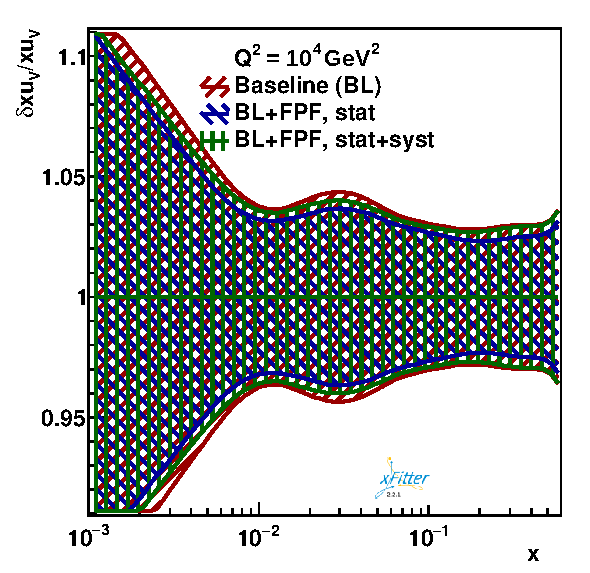
\includegraphics[width=0.32\textwidth]{plots/nuclear_fasernu2/FPF/fred05fcorr05_FPF_q2_10000_pdf_uv_ratio.pdf}
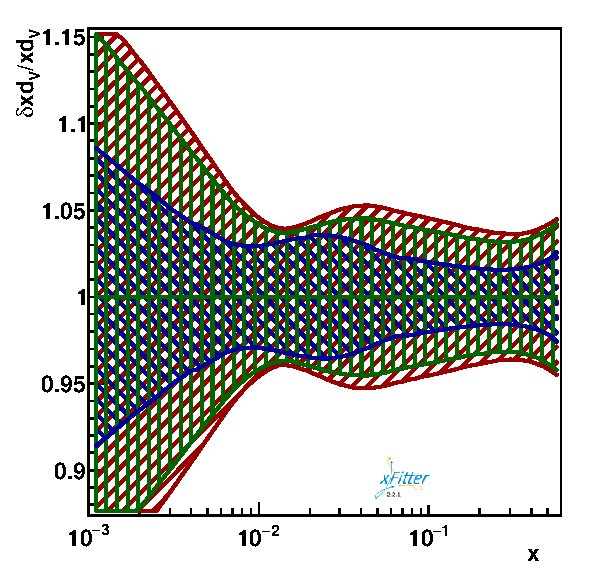
\includegraphics[width=0.32\textwidth]{plots/nuclear_fasernu2/FPF/fred05fcorr05_FPF_q2_10000_pdf_dv_ratio.pdf}
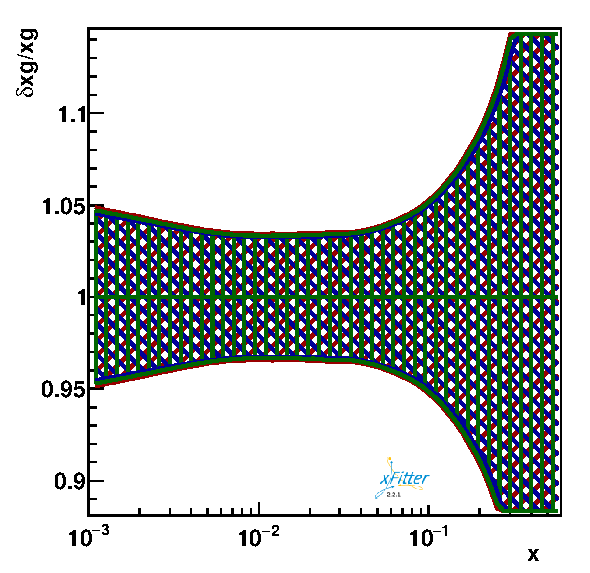
\includegraphics[width=0.32\textwidth]{plots/nuclear_fasernu2/FPF/fred05fcorr05_FPF_q2_10000_pdf_g_ratio.pdf}\\
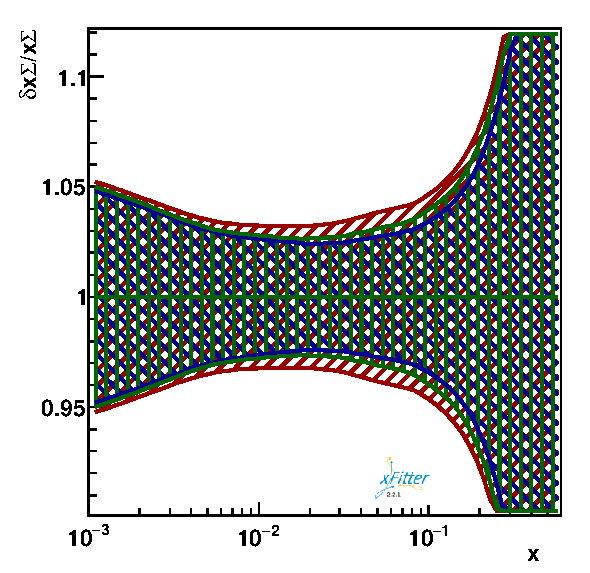
\includegraphics[width=0.32\textwidth]{plots/nuclear_fasernu2/FPF/fred05fcorr05_FPF_q2_10000_pdf_Sea_ratio.pdf}
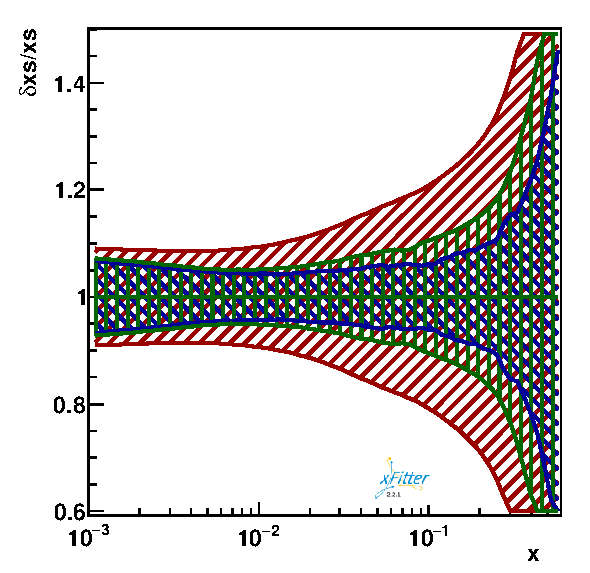
\includegraphics[width=0.32\textwidth]{plots/nuclear_fasernu2/FPF/fred05fcorr05_FPF_q2_10000_pdf_s_ratio.pdf}
\caption{Same as Fig.~\ref{fig:FPF_combined} now corresponding to the Hessian
 profiling of EPPS21 for a tungsten nucleus.
}
\label{fig:profiling_FPF_nuclear}
\end{figure}
%%%%%%%%%%%%%%%%%%%%%%%%%%%%%%%%%%%%%%%%%%%%%%%%%%%%%%%%%%%%%%%%%%%%%%%%

Fig.~\ref{fig:profiling_FPF_nuclear} displays a similar comparison as that of
 Fig.~\ref{fig:FPF_combined}, now corresponding to the Hessian
 profiling of EPPS21 for a tungsten nucleus.
 %
 The FPF dataset is in this case composed by FASER$\nu$2 and AdvSND, given that FLArE
 adopts a different target material.
 %
 Also in this case of nuclear PDFs one finds that the impact of FPF structure function measurements
 is most important for the strange PDF, and to a lesser extent for the up and down
 valence quark PDFs.
 %
 For the latter, the projected impact of FPF measurements appears to be somewhat milder
 as in the case of PDF4LHC21, specially once systematic uncertainties are taken into account.

 While the main qualitative features of the nPDF profiling are consistent with the free-proton
 case, one reason explaining the observed differences is the choice of a larger tolerance factor $T$ in EPPS21
 as compared to PDF4HC21, which effectively reduces the impact of new data.
 %
 Another reason is the more restrictive functional form adopted in EPPS21 as compared
 to the PDF sets entering PDF4LHC21, a consequence of the smaller dataset available
 for hard scattering on nuclear targets.
 %
 Given that these  functional forms are fixed when applying Hessian profiling,
 assessing the impact on a nuclear PDFs by a direct refit, as was done for NNPDF4.0,
 may provide a more  robust estimate of the impact of FPF structure function data
 on nuclear PDFs.
 %
 Additional results for the Hessian profiling of EPPS21 are presented in App.~\ref{app:nPDF_impact_appendix}.
